\card{Aktivitäten während der Anforderungsstufe}{
	\begin{compactenum}
		\item Anfangspunkt: Kundenanforderungen (abstrakt), Systemspezifikationsdokument (Hardware und Software) (SSD)
		\item Aktivitäten:
			\begin{itemize}
				\item Anforderungserhebung (Interviews, Szenarien, Marktbeobachtung, \dots), bestimmen, welche der möglichen widersprüchlichen Anforderungen wichtig sind
				\item Anforderungsdokumentation und -spezifikation (verständliches Anforderungsdokument)
				\item Anforderungsbestätigung (Konsistenz, Vollständigkeit,\\ Übereinstimmung von dokumentierten Anforderungen und den abstrakten Kunden- oder Benutzeranforderungen)
			\end{itemize}
			\item soziale Aktivität: nicht eine einzige Person weiß alles über das System $\Rightarrow$ Kommunikation ist nötig $\Rightarrow$ schwierig (technische Sprache, Unklarheiten, dem Kunden nicht bekannte Anforderungen,\\ Persönlichkeiten)
	\end{compactenum}}

\card{Aktivitäten während der Anforderungsstufe: Diagramm}{
	\usetikzlibrary{trees}
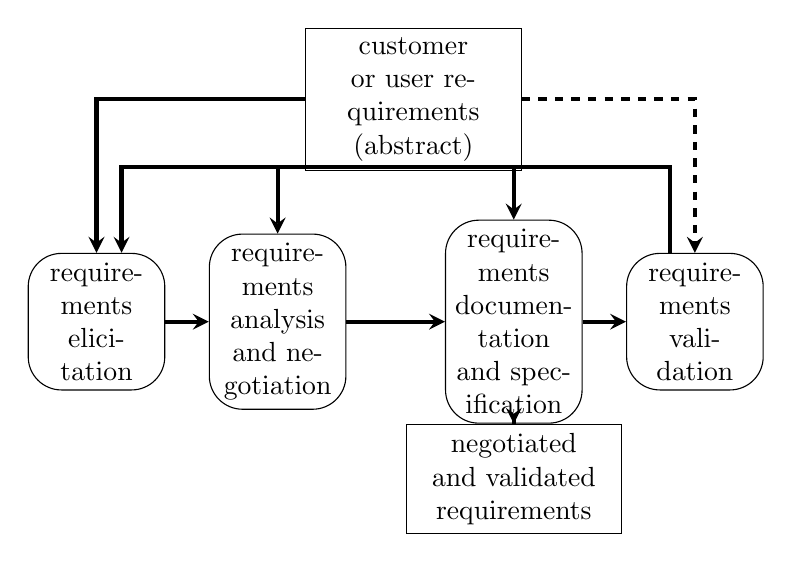
\begin{tikzpicture}[%
	>=stealth,
	node distance=3.5cm,
	auto,
	io/.style={draw, text width=2.5cm, align=center},
	proc/.style={draw, rounded corners=1.2em, text width=1.5cm, align=center},
	dist/.style={node distance = 3cm},
	dick0/.style={draw,line width=1.5pt},
	dick/.style={dick0,->},
	duenn/.style={draw,line width=1.5pt,dashed,->}
]

\node[io] (root) at (0,0) {customer or user requirements (abstract)};

\node[proc] (2) [below left of  = root,xshift=0.75cm,yshift=-0.35cm] {require-ments analysis and negotiation};
\node[proc] (1) [left of       = 2  ,xshift=1.2cm ] {require-ments elicitation};
\node[proc] (3) [below right of = root,xshift=-1.2cm,yshift=-0.35cm] {require-ments documentation and specification};
\node[proc] (4) [right of      = 3  ,xshift=-1.2cm ] {require-ments validation};

\node[io,node distance=2cm] (leaf) [below of = 3] {negotiated and validated requirements};

\node[node distance=1.5cm] (phantom1) [below left of =root,yshift=0.2cm] {};
\node[node distance=1.5cm] (phantom2) [below right of =root,yshift=0.2cm] {};

\path[dick] (root) -| (1);
\path[dick] (1) -- (2);
\path[dick] (2) -- (3);
\path[dick] (3) -- (4);
\path[dick] (3) -- (leaf);
\path[duenn] (root) -| (4);

\path[dick] (phantom2) -| (1.70);
\path[dick] (phantom2) -| (2);
\path[dick] (phantom1) -| (3);
\path[dick0] (phantom1) -| (4.110);


%	\node[state] (A)              {A};
%	\node        (B) [right of=A,fill=blue!25,text width=3cm]{This is a demonstration text for showing how line breaking works.};;
%	\path[->] (A) edge (B);


\end{tikzpicture}
}
